\documentclass[a4paper,12pt]{report}

\usepackage[utf8]{inputenc}
\usepackage[T1]{fontenc}
\usepackage{array}
\usepackage{amsmath}
\usepackage[english]{babel}
\usepackage{graphicx}
\usepackage[a4paper]{geometry}
\usepackage[colorlinks=true,urlcolor=blue,linkcolor=blue]{hyperref}
\usepackage{url}
\usepackage[nottoc,numbib]{tocbibind}
\usepackage{color}
\usepackage{epstopdf}
\usepackage{xcolor}

\makeatletter
	\renewcommand{\thechapter}{\Roman{chapter}}
\makeatother

\begin{document}

\chapter{Dynamics of a single Cr spin in a ZnTe quantum dot}

	\section{Exeperiment configuration}	
	
		\subsection{Experimental setup}
		
	\begin{figure}[h!]
	\begin{center}
		\includegraphics[width=10cm]{../FillingPicture.png}
	\end{center}
	\caption{Complete experimental setup with three lasers, accousto-modulator, finishing either on the monochromator or the diodes.}
	\label{ExpSetup}
	\end{figure}
	
	Lorem ipsum dolor sit amet, consectetur adipiscing elit. Curabitur tortor quam, imperdiet quis facilisis sed, fringilla a quam. Cras ante odio, hendrerit ac ante nec, cursus imperdiet urna. Mauris convallis ultricies purus, nec condimentum erat bibendum vel. Aliquam erat volutpat. Pellentesque condimentum, eros a consequat accumsan, turpis sem euismod nisi, sed fringilla quam turpis sit amet erat. Mauris dictum odio sed nisi dapibus, et molestie mauris rutrum. Praesent convallis dolor in nibh blandit bibendum. Quisque sit amet arcu consectetur lorem luctus venenatis nec quis dui. Aliquam erat volutpat. Aenean auctor elit nec tristique dignissim. Nulla massa mi, efficitur semper ex id, pretium eleifend massa. Vivamus sit amet orci scelerisque, gravida est ut, vulputate odio.
		
		\subsection{Studied dot}
		
	\begin{figure}[h!]
	\begin{center}
		\includegraphics[width=10cm]{../FillingPicture.png}
	\end{center}
	\caption{Studied dot spectra and linear polarization}
	\label{DotSpectra}
	\end{figure}
	
	Lorem ipsum dolor sit amet, consectetur adipiscing elit. Curabitur tortor quam, imperdiet quis facilisis sed, fringilla a quam. Cras ante odio, hendrerit ac ante nec, cursus imperdiet urna. Mauris convallis ultricies purus, nec condimentum erat bibendum vel. Aliquam erat volutpat. Pellentesque condimentum, eros a consequat accumsan, turpis sem euismod nisi, sed fringilla quam turpis sit amet erat. Mauris dictum odio sed nisi dapibus, et molestie mauris rutrum. Praesent convallis dolor in nibh blandit bibendum. Quisque sit amet arcu consectetur lorem luctus venenatis nec quis dui. Aliquam erat volutpat. Aenean auctor elit nec tristique dignissim. Nulla massa mi, efficitur semper ex id, pretium eleifend massa. Vivamus sit amet orci scelerisque, gravida est ut, vulputate odio.
	
	\begin{figure}[h!]
	\begin{center}
		\includegraphics[width=10cm]{../FillingPicture.png}
	\end{center}
	\caption{Spectra with different excitation and detection configurations}
	\label{ExpConfig}
	\end{figure}
	
	Lorem ipsum dolor sit amet, consectetur adipiscing elit. Curabitur tortor quam, imperdiet quis facilisis sed, fringilla a quam. Cras ante odio, hendrerit ac ante nec, cursus imperdiet urna. Mauris convallis ultricies purus, nec condimentum erat bibendum vel. Aliquam erat volutpat. Pellentesque condimentum, eros a consequat accumsan, turpis sem euismod nisi, sed fringilla quam turpis sit amet erat. Mauris dictum odio sed nisi dapibus, et molestie mauris rutrum. Praesent convallis dolor in nibh blandit bibendum. Quisque sit amet arcu consectetur lorem luctus venenatis nec quis dui. Aliquam erat volutpat. Aenean auctor elit nec tristique dignissim. Nulla massa mi, efficitur semper ex id, pretium eleifend massa. Vivamus sit amet orci scelerisque, gravida est ut, vulputate odio.
	
	\section{Cr spin time fluctuations}
	
		\subsection{Autocorrelation: conservation of the Cr spin}
		
	\begin{figure}[h!]
	\begin{center}
		\includegraphics[width=10cm]{../FillingPicture.png}
	\end{center}
	\caption{Autocor of X alone in comparison of X-Cr, and autocor of 3 peaks, and autocor comparison with and without B field}
	\label{AutocorExpCr}
	\end{figure}		
		
		Lorem ipsum dolor sit amet, consectetur adipiscing elit. Curabitur tortor quam, imperdiet quis facilisis sed, fringilla a quam. Cras ante odio, hendrerit ac ante nec, cursus imperdiet urna. Mauris convallis ultricies purus, nec condimentum erat bibendum vel. Aliquam erat volutpat. Pellentesque condimentum, eros a consequat accumsan, turpis sem euismod nisi, sed fringilla quam turpis sit amet erat. Mauris dictum odio sed nisi dapibus, et molestie mauris rutrum. Praesent convallis dolor in nibh blandit bibendum. Quisque sit amet arcu consectetur lorem luctus venenatis nec quis dui. Aliquam erat volutpat. Aenean auctor elit nec tristique dignissim. Nulla massa mi, efficitur semper ex id, pretium eleifend massa. Vivamus sit amet orci scelerisque, gravida est ut, vulputate odio.

	\begin{figure}[h!]
	\begin{center}
		\includegraphics[width=10cm]{../FillingPicture.png}
	\end{center}
	\caption{Autocor power variation effect}
	\label{AutocorPwCr}
	\end{figure}	

	Curabitur eget ipsum egestas dui viverra suscipit. Cras aliquet lacus vitae erat finibus semper. Nulla pharetra eget urna vitae sodales. Nunc faucibus velit lacus, nec ornare eros aliquet quis. Donec a orci nec sem pulvinar ultricies sit amet ut arcu. Nullam id vehicula enim, at tincidunt velit. Duis vestibulum lorem a molestie fringilla. Nullam tincidunt semper placerat. Donec nibh sem, ornare eget cursus ac, luctus sit amet eros. Phasellus eget interdum nisi. Donec mollis risus id lectus fringilla, et commodo risus iaculis. Donec at lacus sed nibh posuere posuere sit amet eget sapien. In dignissim, enim sit amet convallis fermentum, lacus nulla gravida tortor, non facilisis ex nisl sit amet augue. Maecenas eu enim condimentum, consectetur ligula vel, tincidunt nisl. Nam laoreet dictum volutpat. Donec at erat venenatis, ultrices lorem ac, vestibulum neque.
	
		
		\subsection{Cross-correlation: flipping of the Cr spin}
		
		Lorem ipsum dolor sit amet, consectetur adipiscing elit. Curabitur tortor quam, imperdiet quis facilisis sed, fringilla a quam. Cras ante odio, hendrerit ac ante nec, cursus imperdiet urna. Mauris convallis ultricies purus, nec condimentum erat bibendum vel. Aliquam erat volutpat. Pellentesque condimentum, eros a consequat accumsan, turpis sem euismod nisi, sed fringilla quam turpis sit amet erat. Mauris dictum odio sed nisi dapibus, et molestie mauris rutrum. Praesent convallis dolor in nibh blandit bibendum. Quisque sit amet arcu consectetur lorem luctus venenatis nec quis dui. Aliquam erat volutpat. Aenean auctor elit nec tristique dignissim. Nulla massa mi, efficitur semper ex id, pretium eleifend massa. Vivamus sit amet orci scelerisque, gravida est ut, vulputate odio.
		
	\begin{figure}[h!]
	\begin{center}
		\includegraphics[width=10cm]{../FillingPicture.png}
	\end{center}
	\caption{Cross-correlation fitted with exponential, and cross correlation under magnetic field.}
	\label{CrosscorExpCr}
	\end{figure}	
		
	Curabitur eget ipsum egestas dui viverra suscipit. Cras aliquet lacus vitae erat finibus semper. Nulla pharetra eget urna vitae sodales. Nunc faucibus velit lacus, nec ornare eros aliquet quis. Donec a orci nec sem pulvinar ultricies sit amet ut arcu. Nullam id vehicula enim, at tincidunt velit. Duis vestibulum lorem a molestie fringilla. Nullam tincidunt semper placerat. Donec nibh sem, ornare eget cursus ac, luctus sit amet eros. Phasellus eget interdum nisi. Donec mollis risus id lectus fringilla, et commodo risus iaculis. Donec at lacus sed nibh posuere posuere sit amet eget sapien. In dignissim, enim sit amet convallis fermentum, lacus nulla gravida tortor, non facilisis ex nisl sit amet augue. Maecenas eu enim condimentum, consectetur ligula vel, tincidunt nisl. Nam laoreet dictum volutpat. Donec at erat venenatis, ultrices lorem ac, vestibulum neque.
	
	\begin{figure}[h!]
	\begin{center}
		\includegraphics[width=10cm]{../FillingPicture.png}
	\end{center}
	\caption{Cross-correlation under power variation}
	\label{CrosscorPwCr}
	\end{figure}	
	
	Curabitur eget ipsum egestas dui viverra suscipit. Cras aliquet lacus vitae erat finibus semper. Nulla pharetra eget urna vitae sodales. Nunc faucibus velit lacus, nec ornare eros aliquet quis. Donec a orci nec sem pulvinar ultricies sit amet ut arcu. Nullam id vehicula enim, at tincidunt velit. Duis vestibulum lorem a molestie fringilla. Nullam tincidunt semper placerat. Donec nibh sem, ornare eget cursus ac, luctus sit amet eros. Phasellus eget interdum nisi. Donec mollis risus id lectus fringilla, et commodo risus iaculis. Donec at lacus sed nibh posuere posuere sit amet eget sapien. In dignissim, enim sit amet convallis fermentum, lacus nulla gravida tortor, non facilisis ex nisl sit amet augue. Maecenas eu enim condimentum, consectetur ligula vel, tincidunt nisl. Nam laoreet dictum volutpat. Donec at erat venenatis, ultrices lorem ac, vestibulum neque.
	
		\subsection{Model of the spin dynamics}
	
	\begin{figure}[h!]
	\begin{center}
		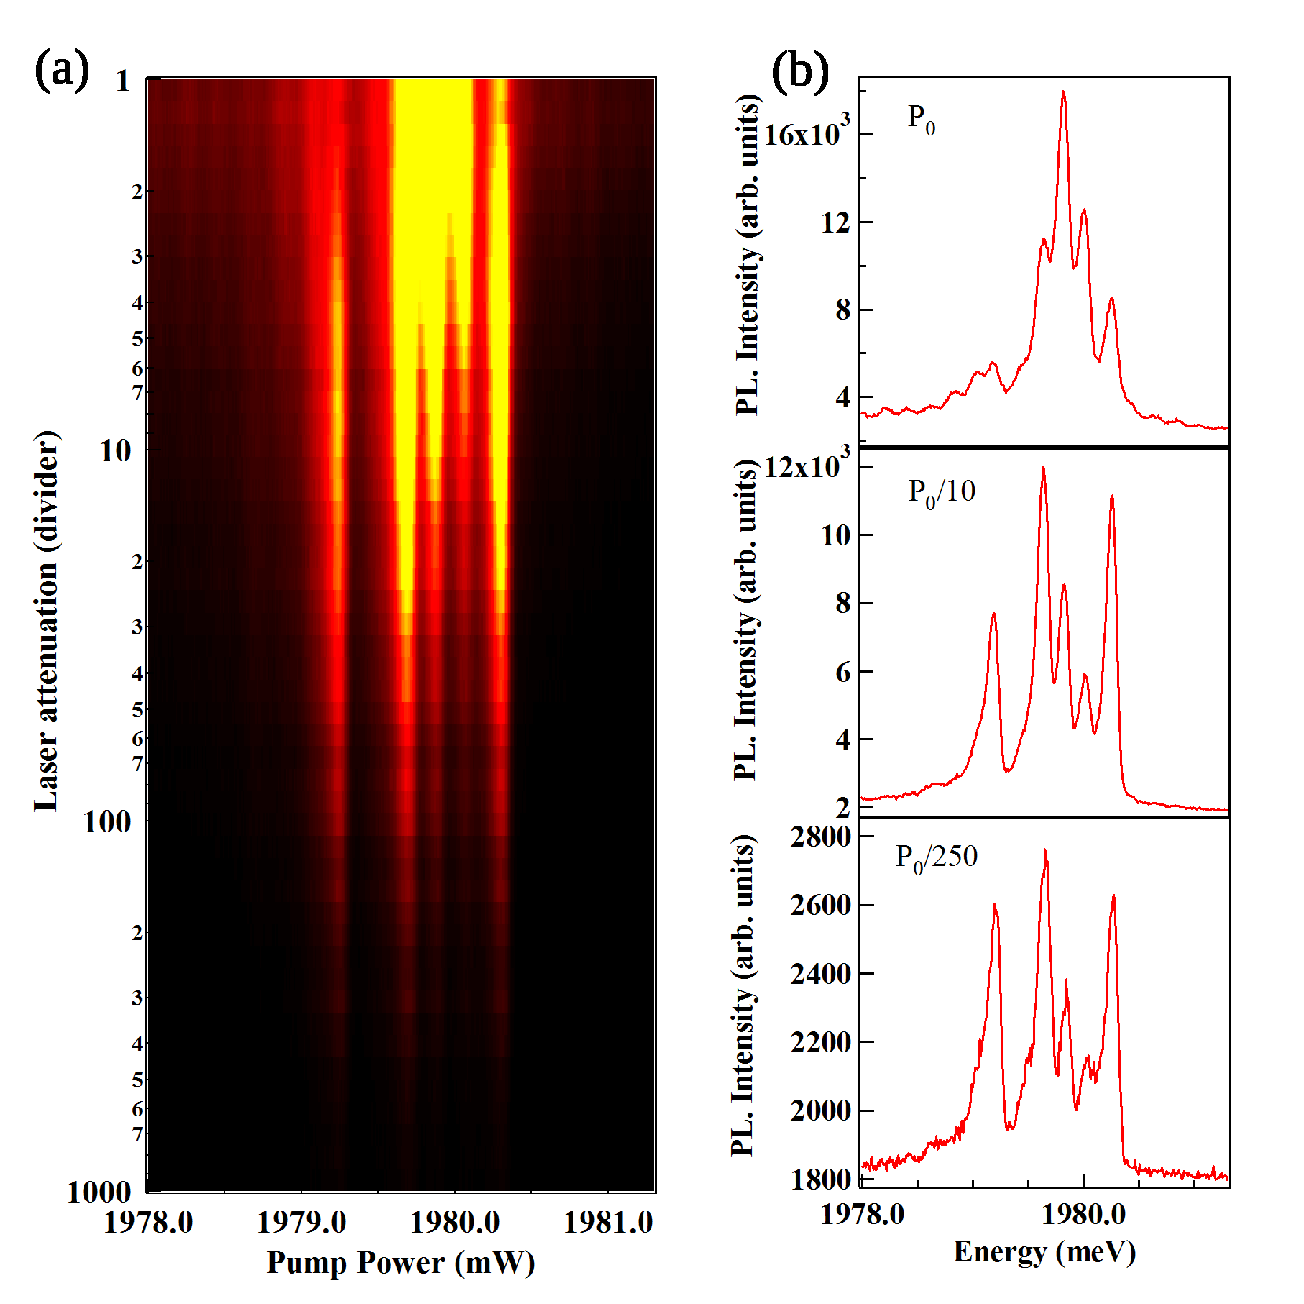
\includegraphics[width=10cm]{Picture/Fig09-PwVar.eps}
	\end{center}
	\caption{Excitation power variations on dot334 QD3 and plot of the intensity of each peak}
	\label{CrSpectraPwExp}
	\end{figure}
	
	In order to study the different relaxation path of the system, probing of the emission evolution under excitation power was realized, reported on Fig.~\ref{CrSpectraPwExp}. As expected, the PL is becoming more intense with the augmentation of the excitation laser, since more exciton are produced and thus injected in the quantum dot. However, this power augmentation response is not the same for each of the peaks. The two central peaks, associated with the $|0\rangle$ states, start at about twice the intensity of the $|\pm1\rangle$ peaks for the most intense one, seemingly never reaching their maximum under our power range. However, when lowering the excitation power, they diminish quickly, and even seems to disappear at low energy, when exterior peaks still show luminescence. Plotting this evolution shows that the two central peaks exhibit a super-linear evolution. On the other side, the exterior peaks begin by rising in intensity before diminishing in a sub-linear fashion. This is coherent with the usual picture, where high power populating preferentially X$^2$-Cr states, while low power populates preferentially X-Cr states~\cite{??}. Finally, one can notice that the dark exciton exhibit the same behaviour, but the maximum emission intensity is at slightly lower power than the $|\pm1\rangle$.

	\begin{figure}[h!]
	\begin{center}
		\includegraphics[width=10cm]{../FillingPicture.png}
	\end{center}
	\caption{Power variation simulation}
	\label{CrSpectraPwMod}
	\end{figure}
	
	The results of this evolution are well reproduced by our spin effective Hamiltonian, using the parameters found for the dot from the magneto-optics and the linear polarization fitting. The model results are presented in Fig.~\ref{CrSpectraPwMod}. [NOT SURE, TO BE REDISCUSSED]The super-linear behaviour of the central peaks can be explained by the proximity of dark exciton states. High power excitation can unlock radiative recombination path to states remaining nonradiative at low excitation power~\cite{PwSuperLinInc}. Such states linked to the $|0\rangle$ state make the emission on its peaks present a super-linear behaviour when excited at high power. 	

	\begin{figure}[h!]
	\begin{center}
		\includegraphics[width=10cm]{../FillingPicture.png}
	\end{center}
	\caption{Simulation of autocorrelation on each peak and cross-correlation |+1> to |-1>}
	\label{SimulCRossAuto}
	\end{figure}			
		
	Lorem ipsum dolor sit amet, consectetur adipiscing elit. Curabitur tortor quam, imperdiet quis facilisis sed, fringilla a quam. Cras ante odio, hendrerit ac ante nec, cursus imperdiet urna. Mauris convallis ultricies purus, nec condimentum erat bibendum vel. Aliquam erat volutpat. Pellentesque condimentum, eros a consequat accumsan, turpis sem euismod nisi, sed fringilla quam turpis sit amet erat. Mauris dictum odio sed nisi dapibus, et molestie mauris rutrum. Praesent convallis dolor in nibh blandit bibendum. Quisque sit amet arcu consectetur lorem luctus venenatis nec quis dui. Aliquam erat volutpat. Aenean auctor elit nec tristique dignissim. Nulla massa mi, efficitur semper ex id, pretium eleifend massa. Vivamus sit amet orci scelerisque, gravida est ut, vulputate odio.
	
	\begin{figure}[h!]
	\begin{center}
		\includegraphics[width=10cm]{../FillingPicture.png}
	\end{center}
	\caption{Autocorrelation simulation with $\tau_Cr$ variations}
	\label{AutocorTauVar}
	\end{figure}	

	Curabitur eget ipsum egestas dui viverra suscipit. Cras aliquet lacus vitae erat finibus semper. Nulla pharetra eget urna vitae sodales. Nunc faucibus velit lacus, nec ornare eros aliquet quis. Donec a orci nec sem pulvinar ultricies sit amet ut arcu. Nullam id vehicula enim, at tincidunt velit. Duis vestibulum lorem a molestie fringilla. Nullam tincidunt semper placerat. Donec nibh sem, ornare eget cursus ac, luctus sit amet eros. Phasellus eget interdum nisi. Donec mollis risus id lectus fringilla, et commodo risus iaculis. Donec at lacus sed nibh posuere posuere sit amet eget sapien. In dignissim, enim sit amet convallis fermentum, lacus nulla gravida tortor, non facilisis ex nisl sit amet augue. Maecenas eu enim condimentum, consectetur ligula vel, tincidunt nisl. Nam laoreet dictum volutpat. Donec at erat venenatis, ultrices lorem ac, vestibulum neque.
	
	\begin{figure}[h!]
	\begin{center}
		\includegraphics[width=10cm]{../FillingPicture.png}
	\end{center}
	\caption{Simulation of autocorrelation and cross-correlation under magnetic field}
	\label{AutoCrosModMagField}
	\end{figure}	
	
	Curabitur eget ipsum egestas dui viverra suscipit. Cras aliquet lacus vitae erat finibus semper. Nulla pharetra eget urna vitae sodales. Nunc faucibus velit lacus, nec ornare eros aliquet quis. Donec a orci nec sem pulvinar ultricies sit amet ut arcu. Nullam id vehicula enim, at tincidunt velit. Duis vestibulum lorem a molestie fringilla. Nullam tincidunt semper placerat. Donec nibh sem, ornare eget cursus ac, luctus sit amet eros. Phasellus eget interdum nisi. Donec mollis risus id lectus fringilla, et commodo risus iaculis. Donec at lacus sed nibh posuere posuere sit amet eget sapien. In dignissim, enim sit amet convallis fermentum, lacus nulla gravida tortor, non facilisis ex nisl sit amet augue. Maecenas eu enim condimentum, consectetur ligula vel, tincidunt nisl. Nam laoreet dictum volutpat. Donec at erat venenatis, ultrices lorem ac, vestibulum neque.
	
	\begin{figure}[h!]
	\begin{center}
		\includegraphics[width=10cm]{../FillingPicture.png}
	\end{center}
	\caption{Simulation of autocorrelation under power variation}
	\label{AutocorPwMod}
	\end{figure}			
	
	\section{Preparation the spin of a Cr atom in a quantum dot}
	
		\subsection{Resonant optical pumping of a spin level}
		
	\begin{figure}[h!]
	\begin{center}
		\includegraphics[width=10cm]{../FillingPicture.png}
	\end{center}
	\caption{Pumping on peak 4}
	\label{PumpCrExp}
	\end{figure}	
	
		Lorem ipsum dolor sit amet, consectetur adipiscing elit. Curabitur tortor quam, imperdiet quis facilisis sed, fringilla a quam. Cras ante odio, hendrerit ac ante nec, cursus imperdiet urna. Mauris convallis ultricies purus, nec condimentum erat bibendum vel. Aliquam erat volutpat. Pellentesque condimentum, eros a consequat accumsan, turpis sem euismod nisi, sed fringilla quam turpis sit amet erat. Mauris dictum odio sed nisi dapibus, et molestie mauris rutrum. Praesent convallis dolor in nibh blandit bibendum. Quisque sit amet arcu consectetur lorem luctus venenatis nec quis dui. Aliquam erat volutpat. Aenean auctor elit nec tristique dignissim. Nulla massa mi, efficitur semper ex id, pretium eleifend massa. Vivamus sit amet orci scelerisque, gravida est ut, vulputate odio.
		
	\begin{figure}[h!]
	\begin{center}
		\includegraphics[width=10cm]{../FillingPicture.png}
	\end{center}
	\caption{3 examples of pumping graphs under different excitation and plot of the variation}
	\label{PumpPwCrExp}
	\end{figure}		

	Curabitur eget ipsum egestas dui viverra suscipit. Cras aliquet lacus vitae erat finibus semper. Nulla pharetra eget urna vitae sodales. Nunc faucibus velit lacus, nec ornare eros aliquet quis. Donec a orci nec sem pulvinar ultricies sit amet ut arcu. Nullam id vehicula enim, at tincidunt velit. Duis vestibulum lorem a molestie fringilla. Nullam tincidunt semper placerat. Donec nibh sem, ornare eget cursus ac, luctus sit amet eros. Phasellus eget interdum nisi. Donec mollis risus id lectus fringilla, et commodo risus iaculis. Donec at lacus sed nibh posuere posuere sit amet eget sapien. In dignissim, enim sit amet convallis fermentum, lacus nulla gravida tortor, non facilisis ex nisl sit amet augue. Maecenas eu enim condimentum, consectetur ligula vel, tincidunt nisl. Nam laoreet dictum volutpat. Donec at erat venenatis, ultrices lorem ac, vestibulum neque.

	\begin{figure}[h!]
	\begin{center}
		\includegraphics[width=10cm]{../FillingPicture.png}
	\end{center}
	\caption{Examples of pumping under detuning with plot of PL maximum intensity variation and of $\delta I/I$}
	\label{AutocorPwMod}
	\end{figure}	

	Curabitur eget ipsum egestas dui viverra suscipit. Cras aliquet lacus vitae erat finibus semper. Nulla pharetra eget urna vitae sodales. Nunc faucibus velit lacus, nec ornare eros aliquet quis. Donec a orci nec sem pulvinar ultricies sit amet ut arcu. Nullam id vehicula enim, at tincidunt velit. Duis vestibulum lorem a molestie fringilla. Nullam tincidunt semper placerat. Donec nibh sem, ornare eget cursus ac, luctus sit amet eros. Phasellus eget interdum nisi. Donec mollis risus id lectus fringilla, et commodo risus iaculis. Donec at lacus sed nibh posuere posuere sit amet eget sapien. In dignissim, enim sit amet convallis fermentum, lacus nulla gravida tortor, non facilisis ex nisl sit amet augue. Maecenas eu enim condimentum, consectetur ligula vel, tincidunt nisl. Nam laoreet dictum volutpat. Donec at erat venenatis, ultrices lorem ac, vestibulum neque.
	
		\subsection{Spin relaxation}
		
	\begin{figure}[h!]
	\begin{center}
		\includegraphics[width=10cm]{../FillingPicture.png}
	\end{center}
	\caption{Dark time variation of pumping with its plot}
	\label{DarkTimeCrExp}
	\end{figure}	
	
	Lorem ipsum dolor sit amet, consectetur adipiscing elit. Curabitur tortor quam, imperdiet quis facilisis sed, fringilla a quam. Cras ante odio, hendrerit ac ante nec, cursus imperdiet urna. Mauris convallis ultricies purus, nec condimentum erat bibendum vel. Aliquam erat volutpat. Pellentesque condimentum, eros a consequat accumsan, turpis sem euismod nisi, sed fringilla quam turpis sit amet erat. Mauris dictum odio sed nisi dapibus, et molestie mauris rutrum. Praesent convallis dolor in nibh blandit bibendum. Quisque sit amet arcu consectetur lorem luctus venenatis nec quis dui. Aliquam erat volutpat. Aenean auctor elit nec tristique dignissim. Nulla massa mi, efficitur semper ex id, pretium eleifend massa. Vivamus sit amet orci scelerisque, gravida est ut, vulputate odio.

	\section{Optical control of the spin of a Cr atom}
		
		Lorem ipsum dolor sit amet, consectetur adipiscing elit. Curabitur tortor quam, imperdiet quis facilisis sed, fringilla a quam. Cras ante odio, hendrerit ac ante nec, cursus imperdiet urna. Mauris convallis ultricies purus, nec condimentum erat bibendum vel. Aliquam erat volutpat. Pellentesque condimentum, eros a consequat accumsan, turpis sem euismod nisi, sed fringilla quam turpis sit amet erat. Mauris dictum odio sed nisi dapibus, et molestie mauris rutrum. Praesent convallis dolor in nibh blandit bibendum. Quisque sit amet arcu consectetur lorem luctus venenatis nec quis dui. Aliquam erat volutpat. Aenean auctor elit nec tristique dignissim. Nulla massa mi, efficitur semper ex id, pretium eleifend massa. Vivamus sit amet orci scelerisque, gravida est ut, vulputate odio.
	
	\begin{figure}[h!]
	\begin{center}
		\includegraphics[width=10cm]{../FillingPicture.png}
	\end{center}
	\caption{Map of peak 4 and 5 under augmentation of the excitation power + line shape with plot of the splitting variation with power}
	\label{OptStarkCrExp}
	\end{figure}		
	
	Curabitur eget ipsum egestas dui viverra suscipit. Cras aliquet lacus vitae erat finibus semper. Nulla pharetra eget urna vitae sodales. Nunc faucibus velit lacus, nec ornare eros aliquet quis. Donec a orci nec sem pulvinar ultricies sit amet ut arcu. Nullam id vehicula enim, at tincidunt velit. Duis vestibulum lorem a molestie fringilla. Nullam tincidunt semper placerat. Donec nibh sem, ornare eget cursus ac, luctus sit amet eros. Phasellus eget interdum nisi. Donec mollis risus id lectus fringilla, et commodo risus iaculis. Donec at lacus sed nibh posuere posuere sit amet eget sapien. In dignissim, enim sit amet convallis fermentum, lacus nulla gravida tortor, non facilisis ex nisl sit amet augue. Maecenas eu enim condimentum, consectetur ligula vel, tincidunt nisl. Nam laoreet dictum volutpat. Donec at erat venenatis, ultrices lorem ac, vestibulum neque.
	
	\begin{figure}[h!]
	\begin{center}
		\includegraphics[width=10cm]{../FillingPicture.png}
	\end{center}
	\caption{Map of peak 4 and 5 under augmentation of the detuning + line shape with plot of the splitting variation with detuning}
	\label{StarkDetuneCrExp}
	\end{figure}	
	
	Curabitur eget ipsum egestas dui viverra suscipit. Cras aliquet lacus vitae erat finibus semper. Nulla pharetra eget urna vitae sodales. Nunc faucibus velit lacus, nec ornare eros aliquet quis. Donec a orci nec sem pulvinar ultricies sit amet ut arcu. Nullam id vehicula enim, at tincidunt velit. Duis vestibulum lorem a molestie fringilla. Nullam tincidunt semper placerat. Donec nibh sem, ornare eget cursus ac, luctus sit amet eros. Phasellus eget interdum nisi. Donec mollis risus id lectus fringilla, et commodo risus iaculis. Donec at lacus sed nibh posuere posuere sit amet eget sapien. In dignissim, enim sit amet convallis fermentum, lacus nulla gravida tortor, non facilisis ex nisl sit amet augue. Maecenas eu enim condimentum, consectetur ligula vel, tincidunt nisl. Nam laoreet dictum volutpat. Donec at erat venenatis, ultrices lorem ac, vestibulum neque.
	
	\begin{figure}[h!]
	\begin{center}
		\includegraphics[width=10cm]{../FillingPicture.png}
	\end{center}
	\caption{Detuning on 1 and 2 while exciting on 5, with experiment configuration}
	\label{DetuneDarkCrExp}
	\end{figure}	

\bibliographystyle{unsrt}
\bibliography{../Bibliography}

\end{document}